\begin{figure}[!h]
  \begin{center}
    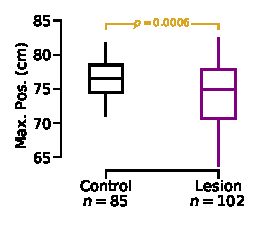
\includegraphics[scale=1]{ch-appendicies/figures/AllRatMaxPos.pdf}
    \caption[Max.\ Pos.\ Comparison]
    {\textbf{Comparing the maximum position for the entire dataset.}
    Each boxplot represents the range of the Max.\ Pos.\ (center line, median; box, 25th and 75th percentiles; whiskers, 5th and 95th percentiles) across a group of animals.
    For every animal, the median value of the last 5 sessions in the control condition (\textit{Control}), or after the striatal lesion (\textit{Lesion}) was considered.
    Comparison using the permutation test (10000 permutations).
    }
    \label{fig:appendix:AllRatMaxPos}
  \end{center}
\end{figure} 